\documentclass[xetex,mathserif,serif]{beamer}
\usepackage{polyglossia}
\setdefaultlanguage[babelshorthands=true]{russian}
\usepackage{minted}
\usepackage{tabu}
\usepackage{algorithm2e}

\useoutertheme{infolines}

\usepackage{fontspec}
\setmainfont{FreeSans}
\newfontfamily{\russianfonttt}{FreeSans}

\setbeamertemplate{blocks}[rounded][shadow=false]

\setbeamercolor*{block title alerted}{fg=red!50!black,bg=red!20}
\setbeamercolor*{block body alerted}{fg=black,bg=red!3}

\tabulinesep=0.5mm

\hypersetup{colorlinks=true, linkcolor=blue, citecolor=blue, filecolor=blue, urlcolor=blue, pdftitle=1, pdfauthor=, pdfsubject=, pdfkeywords=}

\newcommand{\attribution}[1] {
    \begin{flushright}\begin{scriptsize}\textcolor{gray}{#1}\end{scriptsize}\end{flushright}
}

\title{Синтаксический анализ на F\#}
\author{Юрий Литвинов}
\date{17.04.2020г}

\begin{document}
    
    \frame{\titlepage}

    \section{Введение}

    \begin{frame}
        \frametitle{Фазы компиляции}
        \begin{center}
            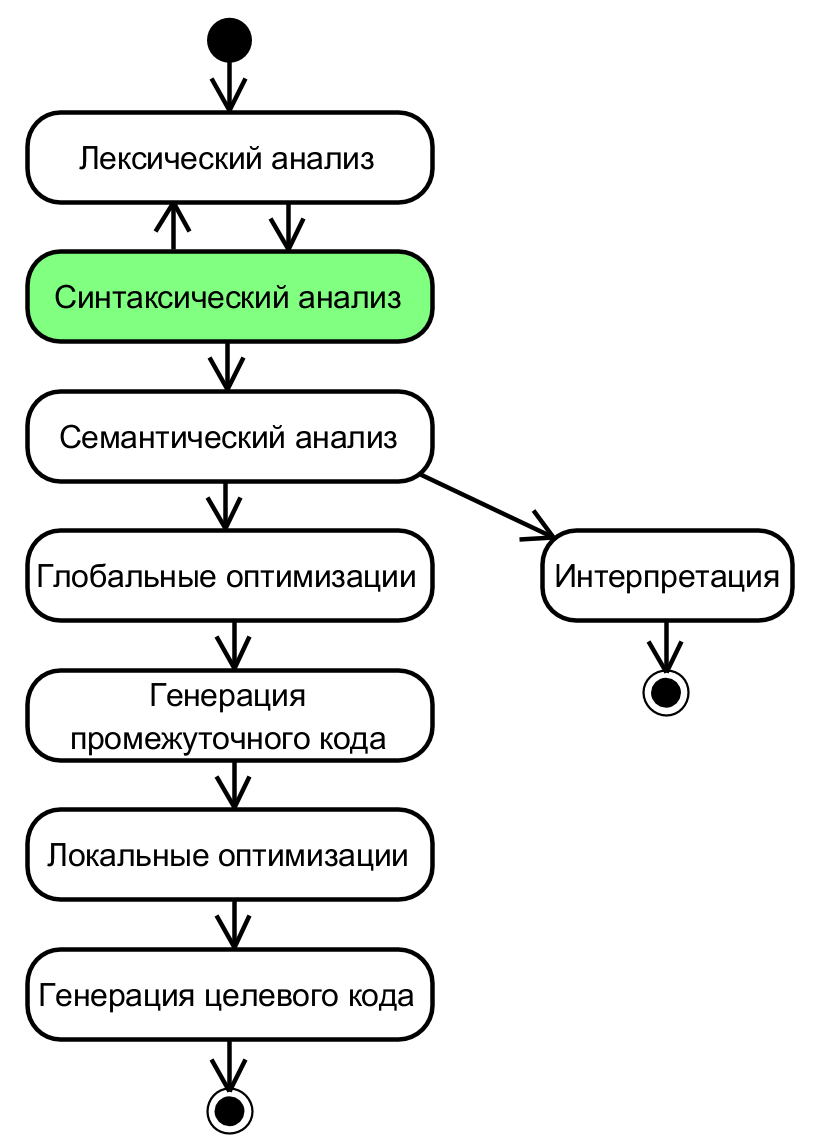
\includegraphics[height=0.8\textheight]{compilerPhases.png}
        \end{center}
    \end{frame}

    \begin{frame}
        \frametitle{Книжка}
        \framesubtitle{Must read}
        \begin{columns}
            \begin{column}{0.6\textwidth}
                А. Ахо, Р. Сети, Дж. Ульман, М. Лам. Компиляторы. Принципы, технологии, инструменты.
                \begin{itemize}
                    \item Так же известна как ``Книга дракона'' (``Dragonbook'')
                \end{itemize}
            \end{column}
            \begin{column}{0.4\textwidth}
                \begin{center}
                    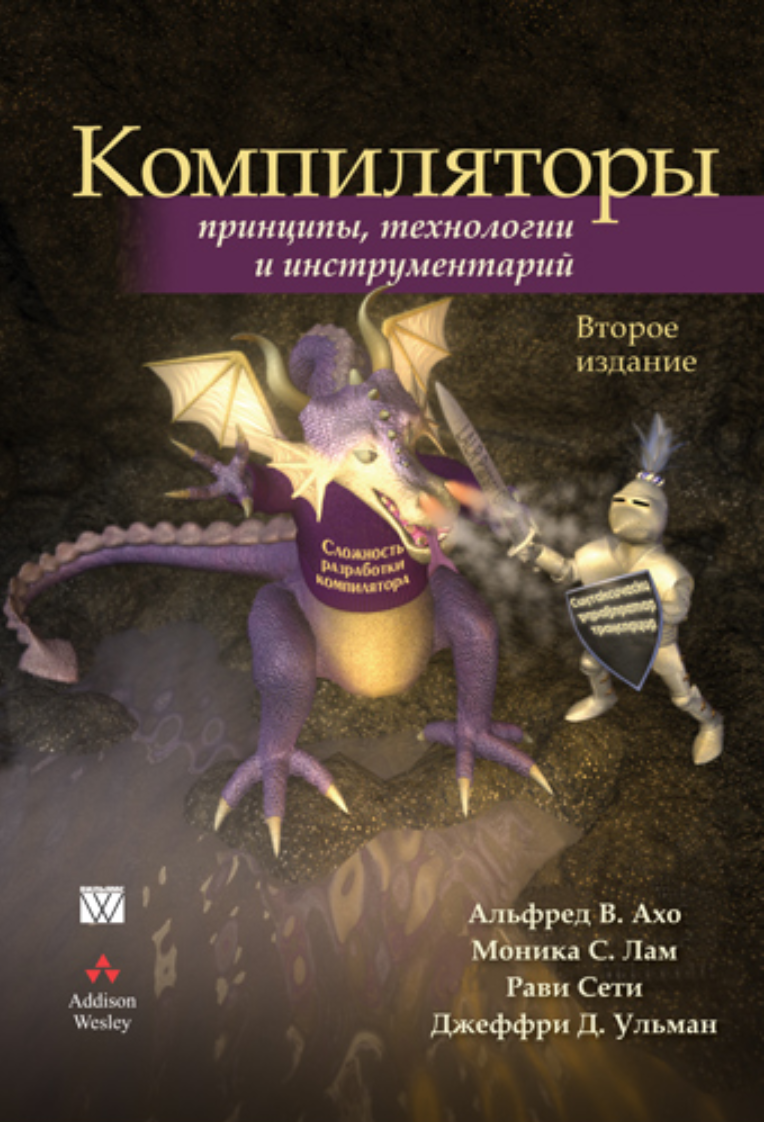
\includegraphics[width=0.7\textwidth]{dragonbook.png}
                \end{center}
            \end{column}
        \end{columns}
    \end{frame}

    \begin{frame}
        \frametitle{Синтаксический анализ}
        \begin{itemize}
            \item Анализ последовательности токенов с целью выяснить синтаксическую структуру
            \begin{itemize}
                \item Сопоставление с формальной грамматикой
            \end{itemize}
            \item Строит структуру данных, представляющую разобранный по синтаксическим правилам документ
            \begin{itemize}
                \item Чаще всего, абстрактное синтаксическое дерево (Abstract Syntax Tree, AST)
                \item Бывает ещё дерево разбора (Parse tree) --- содержит все токены из входной строки, в явном виде обычно не строится
            \end{itemize}
        \end{itemize}
        \begin{center}
            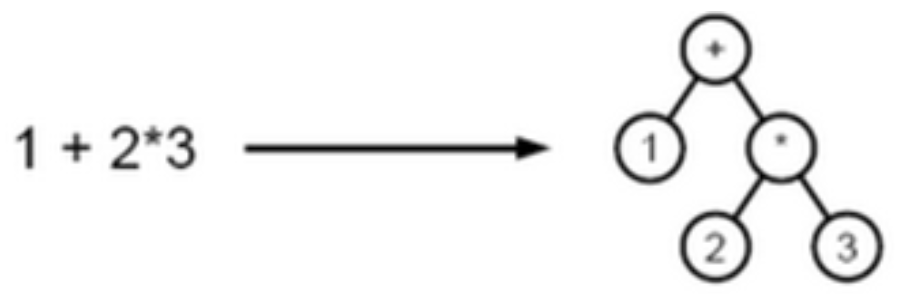
\includegraphics[width=0.4\textwidth]{parsing.png}
        \end{center}
    \end{frame}

    \begin{frame}
        \frametitle{Другие задачи синтаксического анализа}
        \begin{itemize}
            \item Диагностика ошибок
            \item Восстановление после ошибок
            \begin{itemize}
                \item Режим паники
                \item Коррекция
                \item Грамматические правила, обнаруживающие ошибки 
                \begin{itemize}
                    \item ``Предсказание ошибок''
                \end{itemize}
            \end{itemize}
            \item Привязка --- определение для каждой синтаксической конструкции её места в коде
        \end{itemize}
    \end{frame}

    \section{Теория формальных языков}

    \subsection{Формальные грамматики}

    \begin{frame}
        \frametitle{Формальные грамматики}
        \begin{itemize}
            \item Терминал --- символ входной строки для синтаксического анализатора (токен)
            \begin{itemize}
                \item Для лексического анализа входная строка состоит из букв, для синтаксического --- из токенов
            \end{itemize}
            \item Нетерминал --- объект, представляющий сложную синтаксическую конструкцию
            \item Грамматика, формально: $(\Sigma, N, P, S)$, где
            \begin{itemize}
                \item $\Sigma$ --- множество терминалов
                \item $N$ --- множество (алфавит) нетерминальных символов
                \item $P$ --- продукции, функции вида <<цепочка символов>> $\rightarrow$ <<цепочка символов>>, где слева в цепочке есть хотя бы один нетерминал
                \begin{itemize}
                    \item $P: (\Sigma \cup N)^* N (\Sigma \cup N)^* \rightarrow (\Sigma \cup N)^*$
                \end{itemize}
                \item $S$ --- стартовый символ, $S \in N$
            \end{itemize}
        \end{itemize}
    \end{frame}

    \begin{frame}[fragile]
        \frametitle{Пример грамматики}
        \begin{minted}{text}
E ::= E + E
      | E - E
      | -E
      | (E)
      | NUMBER

NUMBER ::= 1 | 2 | 3 | ... | 9
        \end{minted}
    \end{frame}

    \subsection{Иерархия Хомского}

    \begin{frame}
        \frametitle{Иерархия Хомского}
        \begin{itemize}
            \item Регулярные языки (языки типа 3) --- задаются регулярными выражениями, разбираются конечными автоматами
            \item Контекстно-свободные грамматики --- грамматики, у которых слева в продукциях может быть только один символ (нетерминал)
            \begin{itemize}
                \item Пример с предыдущего слайда --- КС-грамматика
                \item Разбираются стековыми автоматами (например, рекурсивным спуском)
            \end{itemize}
            \item Контекстно-зависимые грамматики --- в левой части может быть нетерминал и ``контекст'', нетерминал раскрывается в правой части
            \begin{itemize}
                \item Разбираются линейно ограниченными недетерминированными машинами Тьюринга (то есть, всё плохо)
            \end{itemize}
            \item Языки типа 0 --- грамматики без ограничений на вид продукций
            \begin{itemize}
                \item Разбираются машинами Тьюринга (то есть всё очень плохо)
            \end{itemize}
        \end{itemize}
    \end{frame}

    \begin{frame}
        \frametitle{В реальной жизни}
        \begin{itemize}
            \item Регулярные языки --- регэкспы, весь лексический анализ
            \begin{itemize}
                \item Не умеют считать, поэтому грамматики вида $a^nb^n$ (скобочные последовательности) им не под силу
                \item Не могут в иерархические структуры, никогда не парсите регэкспами HTML
            \end{itemize}
            \item Контекстно-свободные грамматики --- грамматики большинства современных языков программирования
            \begin{itemize}
                \item Не могут в анализ типов
            \end{itemize}
            \item Контекстно-зависимые грамматики --- грамматика C++ и некоторых неаккуратных мест в других языках
            \begin{itemize}
                \item Пример: \mintinline{cpp}|A<B> c;| --- либо \mintinline{cpp}|class A<T> {}|, либо \mintinline{cpp}|int A; int B; int c;|
            \end{itemize}
            \item Языки типа 0 --- естественные языки (да, их тоже анализируют грамматиками, и вообще, Хомский был лингвистом)
        \end{itemize}
    \end{frame}

    \begin{frame}
        \frametitle{Мини-опрос}
        \center{\url{https://forms.gle/BA24ZmgVncH3AP338}}
    \end{frame}

    \subsection{Вывод}

    \begin{frame}
        \frametitle{Вывод в грамматике}
        \begin{itemize}
            \item Формально, если есть грамматика $G = (\Sigma, N, P, S)$, то вывод, $\Rightarrow_G$ --- бинарное отношение на строках
            \begin{itemize}
                \item $x \Rightarrow_G y \iff \exists u, v, p, q \in (\Sigma \cup N)^*: (x = upv) \wedge (p \rightarrow q \in P) \wedge (y = uqv)$
                \item Неформально, шаг вывода --- применение одной из продукций
            \end{itemize}
            \item $\Rightarrow_G^*$ --- рефлексивное транзитивное замыкание $\Rightarrow_G$
            \begin{itemize}
                \item $x \Rightarrow_G^* y$ --- существует конечная последовательность применений продукций грамматики, которая по x делает y
                \item Говорят, <<$y$ выводится из $x$>>
            \end{itemize}
            \item \textit{Порождение} --- последовательность шагов вывода
            \item $L(G)$ --- $\{w \in \Sigma^* | S \Rightarrow_G^* w\}$ --- язык, порождаемый грамматикой $G$
        \end{itemize}
    \end{frame}

    \begin{frame}[fragile]
        \frametitle{Пример}
        Грамматика:
        \begin{minted}{text}
E ::= E + E
      | E * E
      | -E
      | (E)
      | id
        \end{minted}
        
        Входная строка: \mintinline{text}|-(id + id)|
        
        Порождения:
        \begin{itemize}
            \item Левое: \mintinline{text}|E => -E => -(E) => -(E + E) => -(id + E) => -(id + id)|
            \item Правое: \mintinline{text}|E => -E => -(E) => -(E + E) => -(E + id) => -(id + id)|
        \end{itemize}
    \end{frame}

    \subsection{Проблемы грамматик}

    \begin{frame}
        \frametitle{Левая рекурсия}
        \begin{columns}[t]
            \begin{column}{0.5\textwidth}
                Проблема:
                $$A \rightarrow Aa\ |\ b$$
            \end{column}
            \begin{column}{0.5\textwidth}
                Решение: 
                $$A \rightarrow bA'$$
                $$A' \rightarrow aA'\ |\ \epsilon$$
            \end{column}
        \end{columns}
        \begin{columns}[t]
            \begin{column}{0.5\textwidth}
                Пример:
                
                $$E \rightarrow E + T\ |\ T$$
                $$T \rightarrow T * F\ |\ F$$
                $$F \rightarrow (E)\ |\ id$$
            \end{column}
            \begin{column}{0.5\textwidth}
                Пример:

                $$E \rightarrow TE'$$
                $$E' \rightarrow +TE'\ |\ \epsilon$$
                $$T \rightarrow FT'$$
                $$T' \rightarrow *FT\ |\ \epsilon'$$
                $$F \rightarrow (E)\ |\ id$$
            \end{column}
        \end{columns}
    \end{frame}

    \begin{frame}
        \frametitle{Неоднозначность}
        Строка: \mintinline{text}|id + id * id|

        Грамматика (как была): \mintinline{text}!E ::= E + E | E * E | -E | (E) | id!

        Вывод:
        \begin{columns}
            \begin{column}{0.5\textwidth}
                $$E \Rightarrow E + E$$
                $$\Rightarrow id + E$$
                $$\Rightarrow id + E * E$$
                $$\Rightarrow id + id * E$$
                $$\Rightarrow id + id * id$$
                \begin{center}
                    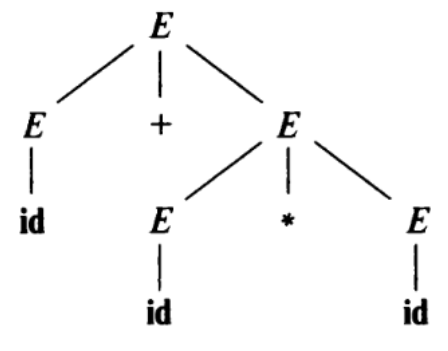
\includegraphics[width=0.5\textwidth]{ambiguousGrammarA.png}
                \end{center}
            \end{column}
            \begin{column}{0.5\textwidth}
                $$E \Rightarrow E * E$$
                $$\Rightarrow E + E * E$$
                $$\Rightarrow id + E * E$$
                $$\Rightarrow id + id * E$$
                $$\Rightarrow id + id * id$$
                \begin{center}
                    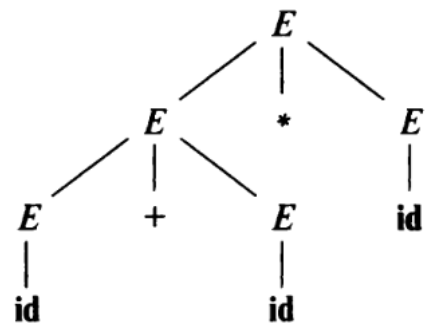
\includegraphics[width=0.5\textwidth]{ambiguousGrammarB.png}
                \end{center}
            \end{column}
        \end{columns}
    \end{frame}

    \subsection{Алгоритмы}

    \begin{frame}
        \frametitle{Алгоритмы разбора}
        \begin{itemize}
            \item Нисходящий разбор --- начинаем со стартового нетерминала, пытаемся построить входную строку
            \begin{itemize}
                \item Рекурсивный спуск
                \item LL-анализ
            \end{itemize}
            \item Восходящий разбор --- пытаемся найти во входной строке последовательность терминалов и нетерминалов и свернуть её в нетерминал
            \begin{itemize}
                \item LR-анализ
            \end{itemize}
        \end{itemize}
    \end{frame}

    \begin{frame}
        \frametitle{Пример}
        \framesubtitle{Нисходящий разбор с построением левого порождения}
        \begin{center}
            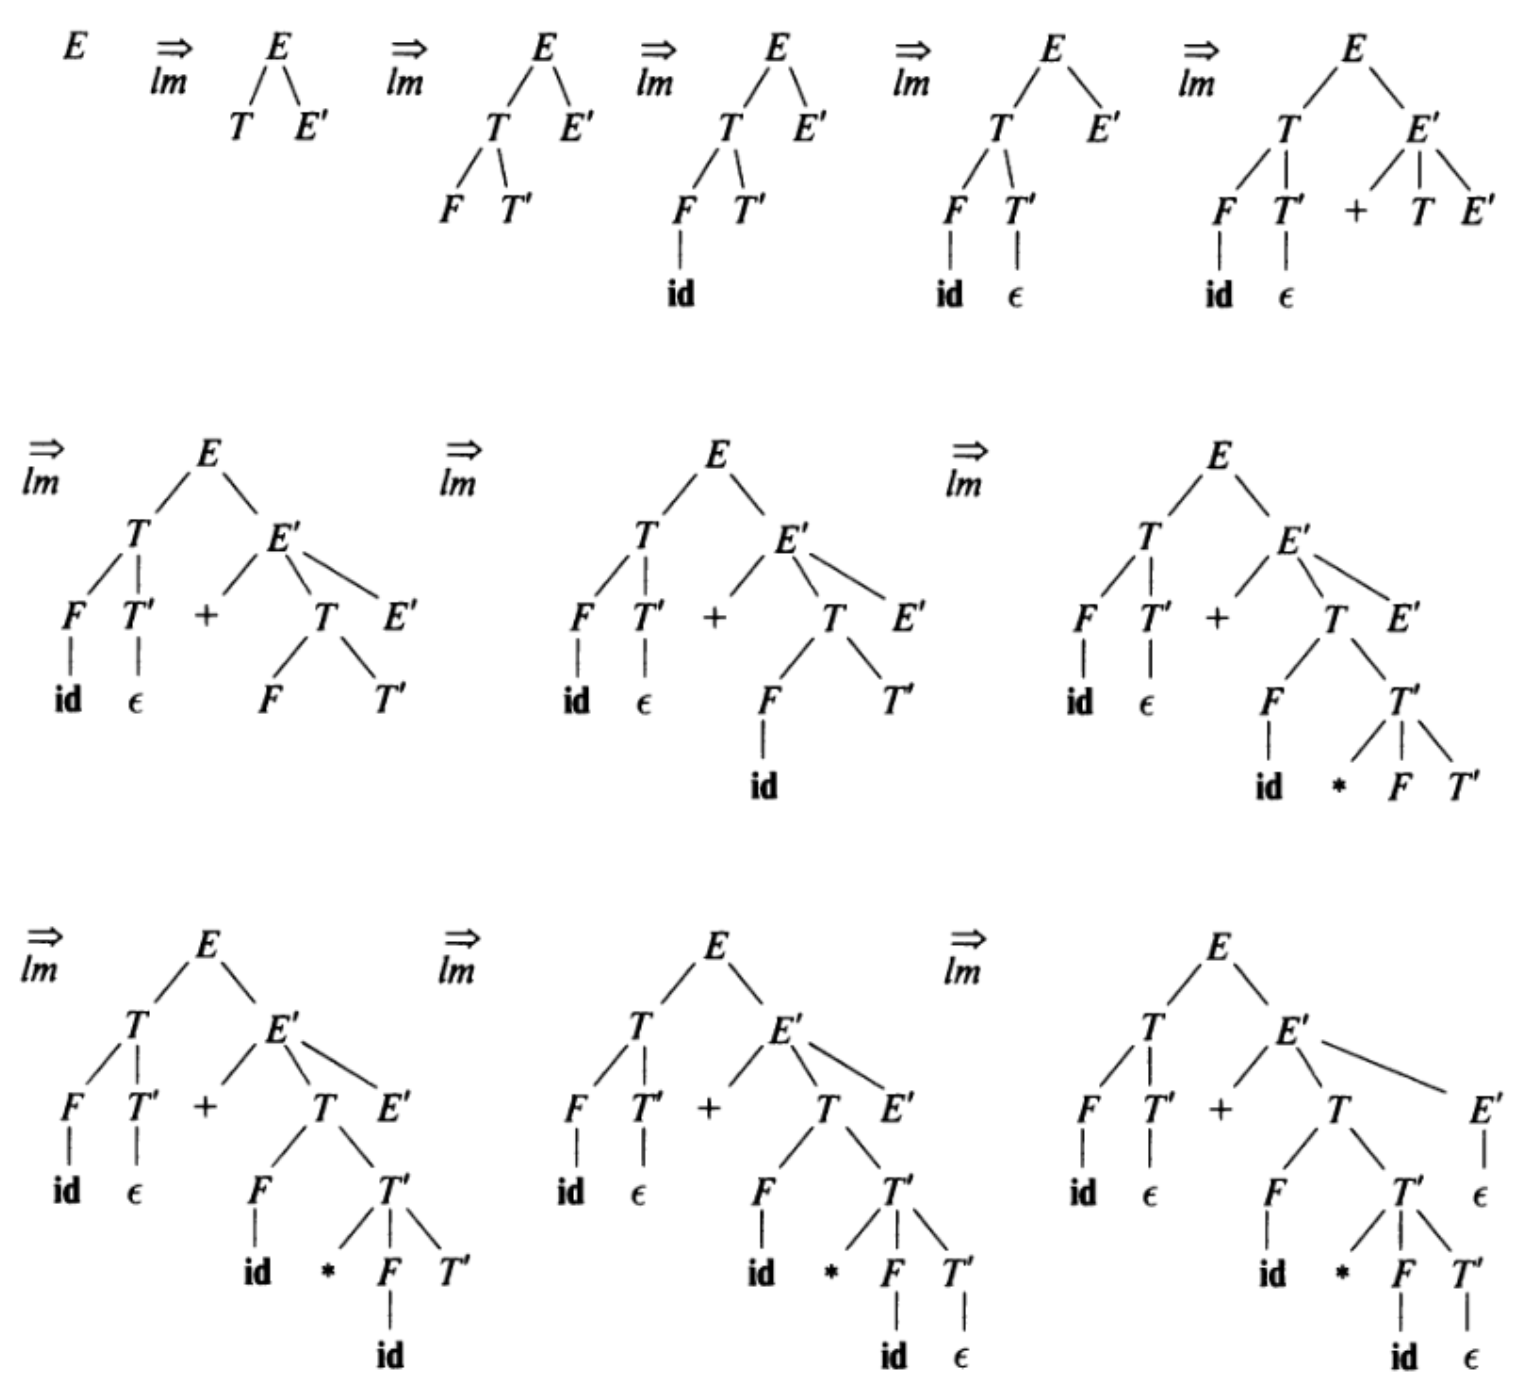
\includegraphics[width=0.65\textwidth]{topDownAnalysis.png}
        \end{center}
    \end{frame}

    \begin{frame}
        \frametitle{FIRST($\alpha$) и FOLLOW($\alpha$)}
        Пусть $\alpha$ --- строка из нетерминалов и терминалов
        \begin{itemize}
            \item FIRST($\alpha$) --- множество всех терминалов, с которых может начинаться $\alpha$
            \begin{itemize}
                \item Считается рекурсивно, раскрытием нетерминальных символов
            \end{itemize}
            \item FOLLOW($\alpha$) --- множество всех терминалов, которые могут стоять за $\alpha$ в выводе в грамматике G
            \begin{itemize}
                \item Считается через FIRST во всех цепочках выводов, в которых может встречаться $\alpha$
                \item $\epsilon$-продукции требуют особого внимания
            \end{itemize}
        \end{itemize}
        Зачем:
        \begin{itemize}
            \item FIRST позволяет выбрать из альтернативных продукций
            \item FOLLOW --- чтобы выбрать между $\epsilon$-продукцией и какой-то другой
        \end{itemize}
    \end{frame}

    \begin{frame}[fragile]
        \frametitle{Рекурсивный спуск}
        \begin{itemize}
            \item По одной функции на нетерминал
            \item Просмотр строки слева направо
        \end{itemize}

        \begin{algorithm}[H]
            Выбираем продукцию $A \rightarrow X_1X_2...X_k$\;
            \For{i от 1 до k}{
                \uIf{$X_i$ -- нетерминал}{
                    Вызов функции $X_i()$\;
                } 
                \uElseIf{$X_i$ равно текущему символу $a$}{
                    Переходим к следующему символу\;
                }
                \Else{
                    Обнаружена ошибка\;
                }
            }
        \end{algorithm}
    \end{frame}

    \subsection{Запись грамматик}

    \begin{frame}
        \frametitle{BNF}
        \framesubtitle{Форма Бэкуса-Наура}
        \begin{itemize}
            \item В угловых скобках --- нетерминал (<literal>)
            \item ::= --- определение (<brackets> ::= '(' | ')')
            \item | --- альтернатива
        \end{itemize}
        Пример: \mintinline{text}/<expr> ::= <term>|<expr><addop><term>/
    \end{frame}

    \begin{frame}[fragile]
        \frametitle{Пример}
        \framesubtitle{BNF, записанная в синтаксисе BNF}
        \begin{footnotesize}
            \begin{minted}{text}
<syntax> ::= <rule> | <rule> <syntax>
<rule> ::= <opt-whitespace> "<" <rule-name> ">" <opt-whitespace> 
        "::=" <opt-whitespace> <expression> <line-end>
<opt-whitespace> ::= " " <opt-whitespace> | ""
<expression> ::= <list> | <list> <opt-whitespace> "|" <opt-whitespace> <expression>
<line-end> ::= <opt-whitespace> <EOL> | <line-end> <line-end>
<list> ::= <term> | <term> <opt-whitespace> <list>
<term> ::= <literal> | "<" <rule-name> ">"
<literal> ::= '"' <text1> '"' | "'" <text2> "'"
<text1> ::= "" | <character1> <text1>
<text2> ::= '' | <character2> <text2>
<character> ::= <letter> | <digit> | <symbol>
<character1> ::= <character> | "'"
<character2> ::= <character> | '"'
<rule-name> ::= <letter> | <rule-name> <rule-char>
<rule-char> ::= <letter> | <digit> | "-"
            \end{minted}
        \end{footnotesize}
    \end{frame}

    \begin{frame}
        \frametitle{Расширенная форма Бэкуса-Наура}
        \begin{itemize}
            \item \{ \} --- 0 или более повторений
            \item {[ ]} --- 0 или 1 раз (опционально)
            \item ( ) --- группировка
            \item , --- конкатенация
            \item Вариантов синтаксиса EBNF больше, чем звёзд на небе
        \end{itemize}
    \end{frame}

    \begin{frame}[fragile]
        \frametitle{Пример}
        \framesubtitle{BNF, записанная в синтаксисе BNF}
        \begin{footnotesize}
            \begin{minted}{text}
character = letter | digit | symbol | "_" ;
identifier = letter , { letter | digit | "_" } ;
terminal = "'" , character , { character } , "'" 
         | '"' , character , { character } , '"' ;
lhs = identifier ;
rhs = identifier
     | terminal
     | "[" , rhs , "]"
     | "{" , rhs , "}"
     | "(" , rhs , ")"
     | rhs , "|" , rhs
     | rhs , "," , rhs ;
rule = lhs , "=" , rhs , ";" ;
grammar = { rule } ;
            \end{minted}
        \end{footnotesize}
    \end{frame}

    \begin{frame}
        \frametitle{Мини-опрос}
        \center{\url{https://forms.gle/6YPGUwKjJxcnwybE8}}
    \end{frame}

    \section{Синтаксический анализ в ФП}

    \subsection{Введение}

    \begin{frame}
        \frametitle{Парсер-комбинаторы}
        \begin{itemize}
            \item Основная идея --- а давайте рассматривать парсер как композицию более простых парсеров
            \begin{itemize}
                \item Определим примитивные парсеры и комбинаторы, строящие парсеры по парсерам
            \end{itemize}
            \item По сути, удобная запись рекурсивного спуска
            \begin{itemize}
                \item Не всегда, иногда используются ``настоящие'' преобразования грамматик
                \begin{itemize}
                    \item Например, Meerkat
                \end{itemize}
            \end{itemize}
            \item Пример --- FParsec
            \begin{itemize}
                \item Порт известной библиотеки Parsec (OCaml)
                \item Рассмотрим \url{http://www.quanttec.com/fparsec/tutorial.html}
            \end{itemize}
        \end{itemize}
    \end{frame}

    \subsection{FParsec}

    \begin{frame}[fragile]
        \frametitle{Пример}
        \begin{minted}{fsharp}
open FParsec

[<EntryPoint>]
let main argv =

    let result = "1.23" |> (run pfloat)

    match result with
    | Success(result, _, _) -> printfn "%f" result
    | Failure(e, _, _) -> printfn "%s" e

    0
        \end{minted}
    \end{frame}

    \begin{frame}[fragile]
        \frametitle{Комбинаторы конкатенации}
        \begin{minted}{fsharp}
val (>>.): Parser<'a,'u> -> Parser<'b,'u> -> Parser<'b,'u>
val (.>>): Parser<'a,'u> -> Parser<'b,'u> -> Parser<'a,'u>

let str s = pstring s
let floatBetweenBrackets = str "[" >>. pfloat .>> str "]"

val pstring: string -> Parser<string,'u>
        \end{minted}
    \end{frame}

    \begin{frame}[fragile]
        \frametitle{Что получилось}
        \begin{small}
            \begin{alertblock}{F\# Interactive}
                \begin{minted}{text}
> test floatBetweenBrackets "[1.0]";;
Success: 1.0

> test floatBetweenBrackets "[]";;
Failure: Error in Ln: 1 Col: 2
[]
 ^
Expecting: floating-point number

> test floatBetweenBrackets "[1.0";;
Failure: Error in Ln: 1 Col: 5
[1.0
    ^
Note: The error occurred at the end of the input stream.
Expecting: ']'
                \end{minted}
            \end{alertblock}
        \end{small}
    \end{frame}

    \begin{frame}[fragile]
        \frametitle{Свои комбинаторы}
        \begin{minted}{fsharp}
let betweenStrings s1 s2 p = str s1 >>. p .>> str s2

let floatBetweenBrackets = pfloat |> betweenStrings "[" "]"
let floatBetweenDoubleBrackets = pfloat |> betweenStrings "[[" "]]"
        \end{minted}

        или

        \begin{minted}{fsharp}
let between pBegin pEnd p  = pBegin >>. p .>> pEnd
let betweenStrings s1 s2 p = p |> between (str s1) (str s2)
        \end{minted}

        between --- библиотечный комбинатор, его определять не надо
    \end{frame}

    \begin{frame}[fragile]
        \frametitle{Разбор списков}
        Грамматика: ("[" float "]")*

        Парсер:
        \begin{alertblock}{F\# Interactive}
            \begin{minted}{text}
> test (many floatBetweenBrackets) "";;
Success: []
> test (many floatBetweenBrackets) "[1.0]";;
Success: [1.0]
> test (many floatBetweenBrackets) "[2][3][4]";;
Success: [2.0; 3.0; 4.0]

> test (many floatBetweenBrackets) "[1][2.0E]";;
Failure: Error in Ln: 1 Col: 9
[1][2.0E]
        ^
Expecting: decimal digit
            \end{minted}
        \end{alertblock}
    \end{frame}

    \begin{frame}[fragile]
        \frametitle{Один или больше элементов}
        Грамматика: ("[" float "]")+

        Парсер:
        \begin{alertblock}{F\# Interactive}
            \begin{minted}{text}
> test (many1 floatBetweenBrackets) "(1)";;
Failure: Error in Ln: 1 Col: 1
(1)
^
Expecting: '['
            \end{minted}
        \end{alertblock}
    \end{frame}

    \begin{frame}[fragile]
        \frametitle{Обработка ошибок}
        \begin{alertblock}{F\# Interactive}
            \begin{minted}{text}
> test (many1 (floatBetweenBrackets 
                          <?> "float between brackets")) "(1)";;
Failure: Error in Ln: 1 Col: 1
(1)
^
Expecting: float between brackets
            \end{minted}
        \end{alertblock}
    \end{frame}

    \begin{frame}[fragile]
        \frametitle{Ещё пример}
        Грамматика: \verb|"[" (float ("," float)*)? "]"|
        
        Примеры: \verb|"[]", "[1.0]", "[2,3,4]"|

        Парсер:
        \begin{minted}{fsharp}
let floatList = str "[" >>. sepBy pfloat (str ",") .>> str "]"
        \end{minted}

        Что получилось:
        \begin{alertblock}{F\# Interactive}
            \begin{minted}{fsharp}
> test floatList "[]";;
Success: []
> test floatList "[1.0]";;
Success: [1.0]
> test floatList "[4,5,6]";;
Success: [4.0; 5.0; 6.0]
            \end{minted}
        \end{alertblock}
    \end{frame}

    \begin{frame}[fragile]
        \frametitle{Пробелы}
        Проблема:
        \begin{alertblock}{F\# Interactive}
            \begin{minted}{fsharp}
> test floatBetweenBrackets "[1.0, 2.0]";;
Failure: Error in Ln: 1 Col: 5
[1.0, 2.0]
       ^
Expecting: ']'
            \end{minted}
        \end{alertblock}
        Решение:
        \begin{minted}{fsharp}
let ws = spaces
let str_ws s = pstring s .>> ws
let float_ws = pfloat .>> ws
let numberList = str_ws "[" >>. sepBy float_ws (str_ws ",") .>> str_ws "]"
        \end{minted}

    \end{frame}

    \begin{frame}[fragile]
        \frametitle{Что получилось}
        \begin{alertblock}{F\# Interactive}
            \begin{minted}{fsharp}
> test numberList @"[ 1 ,
                          2 ] ";;
Success: [1.0; 2.0]

> test numberList @"[ 1,
                         2; 3]";;

Failure: Error in Ln: 2 Col: 27
                         2; 3]
                          ^
Expecting: ',' or ']'
            \end{minted}
        \end{alertblock}
    \end{frame}

    \begin{frame}[fragile]
        \frametitle{Парсинг строк}
        \begin{alertblock}{F\# Interactive}
            \begin{minted}{fsharp}
> test (many (str "a" <|> str "b")) "abba";;
Success: ["a"; "b"; "b"; "a"]

> test (skipStringCI "<float>" >>. pfloat) "<FLOAT>1.0";;
Success: 1.0
            \end{minted}
        \end{alertblock}
        \begin{minted}{fsharp}
let identifier =
    let isIdentifierFirstChar c = isLetter c || c = '_'
    let isIdentifierChar c = isLetter c || isDigit c || c = '_'

    many1Satisfy2L isIdentifierFirstChar isIdentifierChar "identifier"
    .>> ws // skips trailing whitespace
        \end{minted}
        Есть встроенный парсер identifier
    \end{frame}

    \begin{frame}[fragile]
        \frametitle{Строковые литералы}
        \begin{small}
            Грамматика:
            \begin{minted}{text}
stringLiteral: ' " ' (normalChar | escapedChar)* ' " '
normalChar:    any char except '\' and '"'
escapedChar:   '\\' ('\\' | ' " ' | 'n' | 'r' | 't')
            \end{minted}
            Парсер:
            \begin{minted}{fsharp}
let stringLiteral =
    let normalChar = satisfy (fun c -> c <> '\\' && c <> '"')
    let unescape c = match c with
                     | 'n' -> '\n'
                     | 'r' -> '\r'
                     | 't' -> '\t'
                     | c   -> c
    let escapedChar = pstring "\\" >>. (anyOf "\\nrt\"" |>> unescape)
    between (pstring "\"") (pstring "\"")
            (manyChars (normalChar <|> escapedChar))
            \end{minted}
        \end{small}
    \end{frame}

    \begin{frame}[fragile]
        \frametitle{Комбинирование результатов}
        \begin{minted}{fsharp}
val pipe2: Parser<'a,'u> -> Parser<'b,'u> 
                  -> ('a -> b -> 'c) -> Parser<'c,'u>

let product = pipe2 float_ws (str_ws "*" >>. float_ws)
                    (fun x y -> x * y)
        \end{minted}
        Что получилось:
        \begin{alertblock}{F\# Interactive}
            \begin{minted}{text}
> test product "3 * 5";;
Success: 15.0
            \end{minted}
        \end{alertblock}
    \end{frame}

    \begin{frame}[fragile]
        \frametitle{Ещё комбинаторы}
        \begin{minted}{fsharp}
type StringConstant = StringConstant of string * string

let stringConstant = pipe3 identifier (str_ws "=") stringLiteral
                           (fun id _ str -> StringConstant(id, str))
        \end{minted}
        Что получилось:
        \begin{alertblock}{F\# Interactive}
            \begin{minted}{fsharp}
> test stringConstant "myString = \"stringValue\"";;
Success: StringConstant ("myString","stringValue")
            \end{minted}
        \end{alertblock}

        \begin{minted}{fsharp}
fun tuple2 p1 p2 = pipe2 p1 p2 (fun x1 x2 -> (x1, x2))
        \end{minted}

        \begin{alertblock}{F\# Interactive}
            \begin{minted}{fsharp}
> test (float_ws .>>. (str_ws "," >>. float_ws)) "123, 456";;
Success: (123.0, 456.0)
            \end{minted}
        \end{alertblock}
    \end{frame}

    \begin{frame}[fragile]
        \frametitle{Разбор альтернатив}
        \begin{small}
            \begin{minted}{fsharp}
val (<|>): Parser<'a,'u> -> Parser<'a,'u> -> Parser<'a, 'u>

let boolean = (stringReturn "true"  true)
                  <|> (stringReturn "false" false)
            \end{minted}
            Что получилось:
            \begin{alertblock}{F\# Interactive}
                \begin{minted}{text}
> test boolean "false";;
Success: false
> test boolean "true";;
Success: true
> test boolean "tru";;
Failure: Error in Ln: 1 Col: 1
tru
^
Expecting: 'false' or 'true'
                \end{minted}
            \end{alertblock}
        \end{small}
    \end{frame}

    \begin{frame}[fragile]
        \frametitle{Важные особенности}
        \begin{small}
            \begin{itemize}
                \item \verb!<|>! применяет правую часть, только если левая пофэйлилась и не использовала ни один символ из входного потока
                \item \verb!<|>! не делает никакой предпросмотр
                \item \verb!<|>! не ищет самую длинную подходящую строку
            \end{itemize}
            Пример:
            \begin{alertblock}{F\# Interactive}
                \begin{minted}{text}
> run (pstring "a" <|> pstring "ab") "ab";;
val it : ParserResult<string,unit> = Success: "a"

> test ((ws >>. str "a") <|> (ws >>. str "b")) " b";;
Failure: Error in Ln: 1 Col: 2
 b
 ^
Expecting: 'a'
                \end{minted}
            \end{alertblock}
        \end{small}
    \end{frame}

    \begin{frame}[fragile]
        \frametitle{Как пофиксить}
        \begin{alertblock}{F\# Interactive}
            \begin{minted}{text}
> test (ws >>. (str "a" <|> str "b")) " b";;
Success: "b"
            \end{minted}
        \end{alertblock}
    \end{frame}

    \begin{frame}[fragile]
        \frametitle{Ещё комбинаторы}
        \begin{minted}{fsharp}
p1 <|> p2 <|> p3
choice [p1; p2; p3]

val attempt: Parser<'a,'u> -> Parser<'a,'u>
        \end{minted}
        \begin{alertblock}{F\# Interactive}
            \begin{minted}{text}
run ((attempt ab) <|> ac) "ac";;
val it : ParserResult<(string * string),unit> = Success: ("a", "c")
            \end{minted}
        \end{alertblock}
        Комбинаторы бэктрекинга:
        \begin{minted}{fsharp}
val (>>?):  Parser<'a,'u> -> Parser<'b,'u> -> Parser<'b,'u>
(.>>?): Parser<'a,'u> -> Parser<'b,'u> -> Parser<'a,'u>
val (.>>.?): Parser<'a,'u> -> Parser<'b,'u> -> Parser<('a * 'b),'u>
        \end{minted}
    \end{frame}

    \subsection{Парсер JSON}

    \begin{frame}[fragile]
        \frametitle{Большой пример: парсер JSON}
        \begin{itemize}
            \item Грамматика: \url{https://www.json.org/json-en.html}
            \item Пример:
                \begin{minted}{json}
{
    "employee":{ "name":"John", "age":30, "city":"New York" }
    "array": [ "John", "Anna", "Peter" ]
}
                \end{minted}
                \attribution{\url{https://www.w3schools.com/js/js_json_datatypes.asp}}
            \item AST:
                \begin{minted}{fsharp}
type Json = JString of string
          | JNumber of float
          | JBool   of bool
          | JNull
          | JList   of Json list
          | JObject of Map<string, Json>
                \end{minted}
        \end{itemize}
    \end{frame}

    \begin{frame}[fragile]
        \frametitle{Элементарные типы}
        \begin{minted}{fsharp}
let jnull  = stringReturn "null" JNull
let jtrue  = stringReturn "true"  (JBool true)
let jfalse = stringReturn "false" (JBool false)
let jnumber = pfloat |>> JNumber
        \end{minted}
    \end{frame}

    \begin{frame}[fragile]
        \frametitle{Строки}
        \begin{tiny}
            \begin{minted}{fsharp}
let str s = pstring s

let stringLiteral =
    let escape =  anyOf "\"\\/bfnrt"
                  |>> function
                      | 'b' -> "\b"
                      | 'f' -> "\u000C"
                      | 'n' -> "\n"
                      | 'r' -> "\r"
                      | 't' -> "\t"
                      | c   -> string c // every other char is mapped to itself

    let unicodeEscape =
        /// converts a hex char ([0-9a-fA-F]) to its integer number (0-15)
        let hex2int c = (int c &&& 15) + (int c >>> 6)*9

        str "u" >>. pipe4 hex hex hex hex (fun h3 h2 h1 h0 ->
            (hex2int h3)*4096 + (hex2int h2)*256 + (hex2int h1)*16 + hex2int h0
            |> char |> string
        )

    let escapedCharSnippet = str "\\" >>. (escape <|> unicodeEscape)
    let normalCharSnippet  = manySatisfy (fun c -> c <> '"' && c <> '\\')

    between (str "\"") (str "\"")
            (stringsSepBy normalCharSnippet escapedCharSnippet)

let jstring = stringLiteral |>> JString
            \end{minted}
        \end{tiny}
    \end{frame}

    \begin{frame}[fragile]
        \frametitle{Рекурсия}
        \begin{minted}{fsharp}
let jvalue, jvalueRef = createParserForwardedToRef<Json, unit>()
        \end{minted}
        \begin{itemize}
            \item jvalue --- парсер, который просто вызывает парсер из ref-ячейки jvalueRef
            \item Изначально там парсер, который ничего не делает
            \item Поскольку ref-ячейка мутабельна, присвоим туда настоящий парсер позже
        \end{itemize}
    \end{frame}

    \begin{frame}[fragile]
        \frametitle{Списки и объекты}
        \begin{minted}{fsharp}
let ws = spaces
let listBetweenStrings sOpen sClose pElement f =
    between (str sOpen) (str sClose)
            (ws >>. sepBy (pElement .>> ws) (str "," >>. ws) |>> f)
let jlist   = listBetweenStrings "[" "]" jvalue JList

let keyValue = stringLiteral .>>. (ws >>. str ":" >>. ws >>. jvalue)
let jobject = listBetweenStrings "{" "}" keyValue (Map.ofList >> JObject)
        \end{minted}
    \end{frame}

    \begin{frame}[fragile]
        \frametitle{Соберём всё воедино}
        \begin{minted}{fsharp}
do jvalueRef := choice [jobject
                        jlist
                        jstring
                        jnumber
                        jtrue
                        jfalse
                        jnull]

let json = ws >>. jvalue .>> ws .>> eof
        \end{minted}
    \end{frame}

    \subsection{Заключение}

    \begin{frame}
        \frametitle{Заключение}
        \begin{small}
            \begin{itemize}
                \item Подробности: \url{http://www.quanttec.com/fparsec/tutorial.html}
                \item Ещё большие подробности: \url{http://www.quanttec.com/fparsec/users-guide/}
                \item И ещё большие подробности: \url{http://www.quanttec.com/fparsec/reference/}
                \item Осталось за бортом:
                    \begin{itemize}
                        \item FsLex/FsYacc --- неидиоматичный, но более ``взрослый'' генератор парсеров
                            \begin{itemize}
                                \item \url{https://fsprojects.github.io/FsLexYacc/}
                            \end{itemize}
                        \item ANTLR --- стандарт де-факто в серьёзном синтаксическом анализе
                            \begin{itemize}
                                \item \url{https://www.antlr.org/}
                                \item Не поддерживает F\#, но с C\# всё ок
                            \end{itemize}
                        \item YaccConstructor --- мощная библиотека и генератор парсеров, для исследовательских целей
                            \begin{itemize}
                                \item \url{https://github.com/YaccConstructor/YaccConstructor}
                                \item Написан на F\#
                                \item Разрабатывается на матмехе
                            \end{itemize}
                    \end{itemize}
            \end{itemize}
        \end{small}
    \end{frame}

\end{document}
